

\tikzset{every picture/.style={line width=0.75pt}} %set default line width to 0.75pt

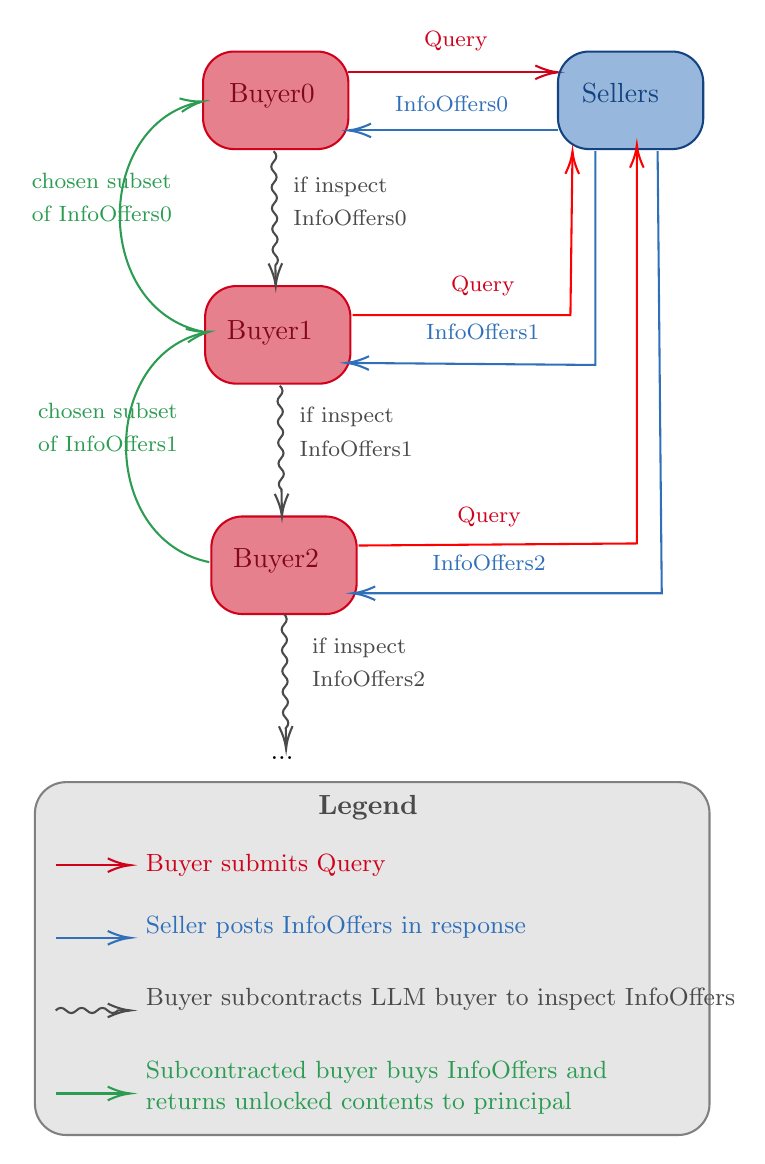
\begin{tikzpicture}[x=0.75pt,y=0.75pt,yscale=-1,xscale=1]
%uncomment if require: \path (0,439); %set diagram left start at 0, and has height of 439

%Straight Lines [id:da41524339668881804]
\draw [color={rgb, 255:red, 208; green, 2; blue, 27 }  ,draw opacity=1 ]   (161,43) -- (260,43) ;
\draw [shift={(262,43)}, rotate = 180] [color={rgb, 255:red, 208; green, 2; blue, 27 }  ,draw opacity=1 ][line width=0.75]    (10.93,-3.29) .. controls (6.95,-1.4) and (3.31,-0.3) .. (0,0) .. controls (3.31,0.3) and (6.95,1.4) .. (10.93,3.29)   ;
%Shape: Rectangle [id:dp2007096083409725]
\draw  [color={rgb, 255:red, 208; green, 2; blue, 27 }  ,draw opacity=1 ][fill={rgb, 255:red, 208; green, 2; blue, 27 }  ,fill opacity=0.5 ] (91,48) .. controls (91,39.72) and (97.72,33) .. (106,33) -- (146,33) .. controls (154.28,33) and (161,39.72) .. (161,48) -- (161,65) .. controls (161,73.28) and (154.28,80) .. (146,80) -- (106,80) .. controls (97.72,80) and (91,73.28) .. (91,65) -- cycle ;
%Shape: Rectangle [id:dp9891337920473939]
\draw  [color={rgb, 255:red, 19; green, 68; blue, 129 }  ,draw opacity=1 ][fill={rgb, 255:red, 48; green, 112; blue, 185 }  ,fill opacity=0.5 ] (262,48) .. controls (262,39.72) and (268.72,33) .. (277,33) -- (317,33) .. controls (325.28,33) and (332,39.72) .. (332,48) -- (332,65) .. controls (332,73.28) and (325.28,80) .. (317,80) -- (277,80) .. controls (268.72,80) and (262,73.28) .. (262,65) -- cycle ;
%Straight Lines [id:da08286653243829956]
\draw [color={rgb, 255:red, 48; green, 112; blue, 185 }  ,draw opacity=1 ]   (262,71) -- (163,71) ;
\draw [shift={(161,71)}, rotate = 360] [color={rgb, 255:red, 48; green, 112; blue, 185 }  ,draw opacity=1 ][line width=0.75]    (10.93,-3.29) .. controls (6.95,-1.4) and (3.31,-0.3) .. (0,0) .. controls (3.31,0.3) and (6.95,1.4) .. (10.93,3.29)   ;
%Shape: Rectangle [id:dp12709317008599474]
\draw  [color={rgb, 255:red, 208; green, 2; blue, 27 }  ,draw opacity=1 ][fill={rgb, 255:red, 208; green, 2; blue, 27 }  ,fill opacity=0.5 ] (92,161) .. controls (92,152.72) and (98.72,146) .. (107,146) -- (147,146) .. controls (155.28,146) and (162,152.72) .. (162,161) -- (162,178) .. controls (162,186.28) and (155.28,193) .. (147,193) -- (107,193) .. controls (98.72,193) and (92,186.28) .. (92,178) -- cycle ;
%Straight Lines [id:da9212547384246598]
\draw [color={rgb, 255:red, 74; green, 74; blue, 74 }  ,draw opacity=1 ]   (125,81) .. controls (126.69,82.64) and (126.72,84.31) .. (125.08,86) .. controls (123.44,87.69) and (123.46,89.35) .. (125.15,91) .. controls (126.84,92.64) and (126.87,94.31) .. (125.23,96) .. controls (123.59,97.69) and (123.62,99.36) .. (125.31,101) .. controls (127,102.65) and (127.02,104.31) .. (125.38,106) .. controls (123.74,107.69) and (123.77,109.36) .. (125.46,111) .. controls (127.15,112.64) and (127.18,114.31) .. (125.54,116) .. controls (123.9,117.69) and (123.93,119.36) .. (125.62,121) .. controls (127.31,122.64) and (127.33,124.3) .. (125.69,125.99) .. controls (124.05,127.68) and (124.08,129.35) .. (125.77,130.99) .. controls (127.46,132.63) and (127.49,134.3) .. (125.85,135.99) -- (125.85,136) -- (125.97,144) ;
\draw [shift={(126,146)}, rotate = 269.12] [color={rgb, 255:red, 74; green, 74; blue, 74 }  ,draw opacity=1 ][line width=0.75]    (10.93,-3.29) .. controls (6.95,-1.4) and (3.31,-0.3) .. (0,0) .. controls (3.31,0.3) and (6.95,1.4) .. (10.93,3.29)   ;
%Curve Lines [id:da5955388933274229]
\draw [color={rgb, 255:red, 43; green, 156; blue, 82 }  ,draw opacity=1 ]   (91,168) .. controls (37.54,157.11) and (37.99,67.81) .. (89.43,57.29) ;
\draw [shift={(91,57)}, rotate = 170.36] [color={rgb, 255:red, 43; green, 156; blue, 82 }  ,draw opacity=1 ][line width=0.75]    (10.93,-3.29) .. controls (6.95,-1.4) and (3.31,-0.3) .. (0,0) .. controls (3.31,0.3) and (6.95,1.4) .. (10.93,3.29)   ;
%Shape: Rectangle [id:dp3154829905272625]
\draw  [color={rgb, 255:red, 208; green, 2; blue, 27 }  ,draw opacity=1 ][fill={rgb, 255:red, 208; green, 2; blue, 27 }  ,fill opacity=0.5 ] (95,272) .. controls (95,263.72) and (101.72,257) .. (110,257) -- (150,257) .. controls (158.28,257) and (165,263.72) .. (165,272) -- (165,289) .. controls (165,297.28) and (158.28,304) .. (150,304) -- (110,304) .. controls (101.72,304) and (95,297.28) .. (95,289) -- cycle ;
%Straight Lines [id:da3417537956466643]
\draw [color={rgb, 255:red, 74; green, 74; blue, 74 }  ,draw opacity=1 ]   (128,194) .. controls (129.69,195.64) and (129.72,197.31) .. (128.08,199) .. controls (126.44,200.69) and (126.47,202.36) .. (128.16,204) .. controls (129.85,205.64) and (129.88,207.31) .. (128.24,209) .. controls (126.6,210.69) and (126.63,212.36) .. (128.32,214) .. controls (130.01,215.64) and (130.04,217.31) .. (128.4,219) .. controls (126.76,220.69) and (126.79,222.36) .. (128.48,224) .. controls (130.17,225.64) and (130.2,227.31) .. (128.56,229) .. controls (126.92,230.69) and (126.94,232.35) .. (128.63,233.99) .. controls (130.32,235.63) and (130.35,237.3) .. (128.71,238.99) .. controls (127.07,240.68) and (127.1,242.35) .. (128.79,243.99) -- (128.84,247) -- (128.97,255) ;
\draw [shift={(129,257)}, rotate = 269.09] [color={rgb, 255:red, 74; green, 74; blue, 74 }  ,draw opacity=1 ][line width=0.75]    (10.93,-3.29) .. controls (6.95,-1.4) and (3.31,-0.3) .. (0,0) .. controls (3.31,0.3) and (6.95,1.4) .. (10.93,3.29)   ;
%Curve Lines [id:da391924904621877]
\draw [color={rgb, 255:red, 43; green, 156; blue, 82 }  ,draw opacity=1 ]   (94,279) .. controls (40.54,268.11) and (40.99,178.81) .. (92.43,168.29) ;
\draw [shift={(94,168)}, rotate = 170.36] [color={rgb, 255:red, 43; green, 156; blue, 82 }  ,draw opacity=1 ][line width=0.75]    (10.93,-3.29) .. controls (6.95,-1.4) and (3.31,-0.3) .. (0,0) .. controls (3.31,0.3) and (6.95,1.4) .. (10.93,3.29)   ;
%Straight Lines [id:da3637784039757481]
\draw [color={rgb, 255:red, 74; green, 74; blue, 74 }  ,draw opacity=1 ]   (130,304) .. controls (131.69,305.64) and (131.72,307.31) .. (130.08,309) .. controls (128.44,310.69) and (128.46,312.35) .. (130.15,314) .. controls (131.84,315.64) and (131.87,317.31) .. (130.23,319) .. controls (128.59,320.69) and (128.62,322.36) .. (130.31,324) .. controls (132,325.65) and (132.02,327.31) .. (130.38,329) .. controls (128.74,330.69) and (128.77,332.36) .. (130.46,334) .. controls (132.15,335.64) and (132.18,337.31) .. (130.54,339) .. controls (128.9,340.69) and (128.93,342.36) .. (130.62,344) .. controls (132.31,345.64) and (132.33,347.3) .. (130.69,348.99) .. controls (129.05,350.68) and (129.08,352.35) .. (130.77,353.99) .. controls (132.46,355.63) and (132.49,357.3) .. (130.85,358.99) -- (130.85,359) -- (130.97,367) ;
\draw [shift={(131,369)}, rotate = 269.12] [color={rgb, 255:red, 74; green, 74; blue, 74 }  ,draw opacity=1 ][line width=0.75]    (10.93,-3.29) .. controls (6.95,-1.4) and (3.31,-0.3) .. (0,0) .. controls (3.31,0.3) and (6.95,1.4) .. (10.93,3.29)   ;
%Straight Lines [id:da5447878474416243]
\draw [color={rgb, 255:red, 255; green, 0; blue, 0 }  ,draw opacity=1 ]   (163,160) -- (268,160) -- (268.97,83) ;
\draw [shift={(269,81)}, rotate = 90.73] [color={rgb, 255:red, 255; green, 0; blue, 0 }  ,draw opacity=1 ][line width=0.75]    (10.93,-3.29) .. controls (6.95,-1.4) and (3.31,-0.3) .. (0,0) .. controls (3.31,0.3) and (6.95,1.4) .. (10.93,3.29)   ;
%Straight Lines [id:da3778704064531401]
\draw [color={rgb, 255:red, 255; green, 0; blue, 0 }  ,draw opacity=1 ]   (166,271) -- (300,270) -- (300,80) ;
\draw [shift={(300,78)}, rotate = 90] [color={rgb, 255:red, 255; green, 0; blue, 0 }  ,draw opacity=1 ][line width=0.75]    (10.93,-3.29) .. controls (6.95,-1.4) and (3.31,-0.3) .. (0,0) .. controls (3.31,0.3) and (6.95,1.4) .. (10.93,3.29)   ;
%Straight Lines [id:da28955812841585316]
\draw [color={rgb, 255:red, 48; green, 112; blue, 185 }  ,draw opacity=1 ]   (280,81) -- (280,184) -- (162,183.02) ;
\draw [shift={(160,183)}, rotate = 0.48] [color={rgb, 255:red, 48; green, 112; blue, 185 }  ,draw opacity=1 ][line width=0.75]    (10.93,-3.29) .. controls (6.95,-1.4) and (3.31,-0.3) .. (0,0) .. controls (3.31,0.3) and (6.95,1.4) .. (10.93,3.29)   ;
%Straight Lines [id:da7668238798267074]
\draw [color={rgb, 255:red, 48; green, 112; blue, 185 }  ,draw opacity=1 ]   (310,81) -- (312,294) -- (165,294) ;
\draw [shift={(163,294)}, rotate = 360] [color={rgb, 255:red, 48; green, 112; blue, 185 }  ,draw opacity=1 ][line width=0.75]    (10.93,-3.29) .. controls (6.95,-1.4) and (3.31,-0.3) .. (0,0) .. controls (3.31,0.3) and (6.95,1.4) .. (10.93,3.29)   ;

%Shape: Legend Rectangle [id:dp5647832748705617] - repositioned below diagram
\draw  [color={rgb, 255:red, 128; green, 128; blue, 128 }  ,draw opacity=1 ][fill={rgb, 255:red, 155; green, 155; blue, 155 }  ,fill opacity=0.25 ] (10,400) .. controls (10,391.72) and (16.72,385) .. (25,385) -- (320,385) .. controls (328.28,385) and (335,391.72) .. (335,400) -- (335,540) .. controls (335,548.28) and (328.28,555) .. (320,555) -- (25,555) .. controls (16.72,555) and (10,548.28) .. (10,540) -- cycle ;

% Legend Title
\draw (145,390) node [anchor=north west][inner sep=0.75pt]  [color={rgb, 255:red, 74; green, 74; blue, 74 }  ,opacity=1 ] [align=left] {\textbf{Legend}};

% Legend Row 1, Item 1: Red arrow - Buyer submits Query
\draw [color={rgb, 255:red, 208; green, 2; blue, 27 }  ,draw opacity=1 ]   (20,425) -- (54,425) ;
\draw [shift={(56,425)}, rotate = 180] [color={rgb, 255:red, 208; green, 2; blue, 27 }  ,draw opacity=1 ][line width=0.75]    (10.93,-3.29) .. controls (6.95,-1.4) and (3.31,-0.3) .. (0,0) .. controls (3.31,0.3) and (6.95,1.4) .. (10.93,3.29)   ;
\draw (62,418) node [anchor=north west][inner sep=0.75pt]  [font=\small,color={rgb, 255:red, 208; green, 2; blue, 27 }  ,opacity=1 ] [align=left] {Buyer submits Query};

% Legend Row 1, Item 2: Blue arrow - Seller posts InfoOffers
\draw [color={rgb, 255:red, 48; green, 112; blue, 185 }  ,draw opacity=1 ]   (54,460) -- (20,460) ;
\draw [shift={(56,460)}, rotate = 180] [color={rgb, 255:red, 48; green, 112; blue, 185 }  ,draw opacity=1 ][line width=0.75]    (10.93,-3.29) .. controls (6.95,-1.4) and (3.31,-0.3) .. (0,0) .. controls (3.31,0.3) and (6.95,1.4) .. (10.93,3.29)   ;
\draw (62,448) node [anchor=north west][inner sep=0.75pt]  [font=\small,color={rgb, 255:red, 48; green, 112; blue, 185 }  ,opacity=1 ] [align=left] {Seller posts InfoOffers in response};

% Legend Row 2, Item 1: Gray wavy arrow - Buyer subcontracts
\draw [color={rgb, 255:red, 74; green, 74; blue, 74 }  ,draw opacity=1 ]   (20,495) .. controls (21.67,493.33) and (23.33,493.33) .. (25,495) .. controls (26.67,496.67) and (28.33,496.67) .. (30,495) .. controls (31.67,493.33) and (33.33,493.33) .. (35,495) .. controls (36.67,496.67) and (38.33,496.67) .. (40,495) .. controls (41.67,493.33) and (43.33,493.33) .. (45,495) .. controls (46.67,496.67) and (48.33,496.67) .. (50,495) -- (54,495) ;
\draw [shift={(56,495)}, rotate = 180] [color={rgb, 255:red, 74; green, 74; blue, 74 }  ,draw opacity=1 ][line width=0.75]    (10.93,-3.29) .. controls (6.95,-1.4) and (3.31,-0.3) .. (0,0) .. controls (3.31,0.3) and (6.95,1.4) .. (10.93,3.29)   ;
\draw (62,483) node [anchor=north west][inner sep=0.75pt]  [font=\small,color={rgb, 255:red, 74; green, 74; blue, 74 }  ,opacity=1 ] [align=left] {Buyer subcontracts LLM buyer to inspect InfoOffers};

% Legend Row 2, Item 2: Green arrow - Subcontracted buyer buys
\draw [color={rgb, 255:red, 43; green, 156; blue, 82 }  ,draw opacity=1 ]   (20,535) -- (54,535) ;
\draw [shift={(56,535)}, rotate = 180] [color={rgb, 255:red, 43; green, 156; blue, 82 }  ,draw opacity=1 ][line width=0.75]    (10.93,-3.29) .. controls (6.95,-1.4) and (3.31,-0.3) .. (0,0) .. controls (3.31,0.3) and (6.95,1.4) .. (10.93,3.29)   ;
\draw (62,518) node [anchor=north west][inner sep=0.75pt]  [font=\small,color={rgb, 255:red, 43; green, 156; blue, 82 }  ,opacity=1 ] [align=left] {Subcontracted buyer buys InfoOffers and\\returns unlocked contents to principal};
% Text Node
\draw (102,47) node [anchor=north west][inner sep=0.75pt]  [color={rgb, 255:red, 129; green, 8; blue, 23 }  ,opacity=1 ] [align=left] {Buyer0};
% Text Node
\draw (272,47) node [anchor=north west][inner sep=0.75pt]  [color={rgb, 255:red, 19; green, 68; blue, 129 }  ,opacity=1 ] [align=left] {Sellers};
% Text Node
\draw (196,22) node [anchor=north west][inner sep=0.75pt]  [color={rgb, 255:red, 208; green, 2; blue, 27 }  ,opacity=1 ] [align=left] {{\footnotesize Query}};
% Text Node
\draw (182,53) node [anchor=north west][inner sep=0.75pt]  [color={rgb, 255:red, 48; green, 112; blue, 185 }  ,opacity=1 ] [align=left] {{\footnotesize InfoOffers0}};
% Text Node
\draw (101,161) node [anchor=north west][inner sep=0.75pt]  [color={rgb, 255:red, 129; green, 8; blue, 23 }  ,opacity=1 ] [align=left] {Buyer1};
% Text Node
\draw (133,92) node [anchor=north west][inner sep=0.75pt]  [color={rgb, 255:red, 74; green, 74; blue, 74 }  ,opacity=1 ] [align=left] {{\footnotesize if inspect}\\{\footnotesize InfoOffers0}};
% Text Node
\draw (209,140) node [anchor=north west][inner sep=0.75pt]  [color={rgb, 255:red, 208; green, 2; blue, 27 }  ,opacity=1 ] [align=left] {{\footnotesize Query}};
% Text Node
\draw (197,163) node [anchor=north west][inner sep=0.75pt]  [color={rgb, 255:red, 48; green, 112; blue, 185 }  ,opacity=1 ] [align=left] {{\footnotesize InfoOffers1}};
% Text Node
\draw (7,90) node [anchor=north west][inner sep=0.75pt]  [color={rgb, 255:red, 43; green, 156; blue, 82 }  ,opacity=1 ] [align=left] {{\footnotesize chosen subset}\\{\footnotesize of InfoOffers0}};
% Text Node
\draw (104,271) node [anchor=north west][inner sep=0.75pt]  [color={rgb, 255:red, 129; green, 8; blue, 23 }  ,opacity=1 ] [align=left] {Buyer2};
% Text Node
\draw (136,203) node [anchor=north west][inner sep=0.75pt]  [color={rgb, 255:red, 74; green, 74; blue, 74 }  ,opacity=1 ] [align=left] {{\footnotesize if inspect}\\{\footnotesize InfoOffers1}};
% Text Node
\draw (212,251) node [anchor=north west][inner sep=0.75pt]  [color={rgb, 255:red, 208; green, 2; blue, 27 }  ,opacity=1 ] [align=left] {{\footnotesize Query}};
% Text Node
\draw (200,274) node [anchor=north west][inner sep=0.75pt]  [color={rgb, 255:red, 48; green, 112; blue, 185 }  ,opacity=1 ] [align=left] {{\footnotesize InfoOffers2}};
% Text Node
\draw (10,201) node [anchor=north west][inner sep=0.75pt]  [color={rgb, 255:red, 43; green, 156; blue, 82 }  ,opacity=1 ] [align=left] {{\footnotesize chosen subset}\\{\footnotesize of InfoOffers1}};
% Text Node
\draw (142,314) node [anchor=north west][inner sep=0.75pt]  [color={rgb, 255:red, 74; green, 74; blue, 74 }  ,opacity=1 ] [align=left] {{\footnotesize if inspect}\\{\footnotesize InfoOffers2}};
% Text Node
\draw (122,371) node [anchor=north west][inner sep=0.75pt]   [align=left] {...};


\end{tikzpicture}
